% !TEX encoding = UTF-8 Unicode
% !TEX spellcheck = en_US

%
\documentclass[runningheads]{llncs}
%
\usepackage[T1]{fontenc}
\usepackage[utf8]{inputenc}
\usepackage{graphicx}
\graphicspath{{./figures/}}
\usepackage{paralist} % for compactitem
\usepackage{amsmath} % for math symbols like \int
\usepackage{nicefrac}
\usepackage{siunitx}
\usepackage{url}
\usepackage{todonotes}
% If you use the hyperref package, please uncomment the following two lines
% to display URLs in blue roman font according to Springer's eBook style:
\usepackage{color}
\renewcommand\UrlFont{\color{blue}\rmfamily}
%%% Custom commands
\newcommand{\bm}[1]{\boldsymbol{#1}}
% Depending on the latex version, vec makes bold font (desired in paper) or arrow over symbol. Therefore redefine here.
\renewcommand{\vec}[1]{\boldsymbol{#1}}
\DeclareMathOperator*{\argmin}{argmin}
\newcommand{\rotmat}[2]{{{ }^{#1}\boldsymbol{R}}_{#2}}
\newcommand{\transp}[0]{{\mathrm{T}}}
%
\begin{document}
%
\title{Pose Optimization of Task-Redundant Robots in Second-Order Rest-to-Rest Motion with Cascaded Dynamic Programming and Nullspace Projection}
%
\titlerunning{Dynamic Programming and Nullspace Projection for Task Redundancy}
\author{Moritz Schappler\inst{1}\orcidID{0000-0001-7952-7363}}
%
\authorrunning{M. Schappler.}
%
\institute{Leibniz University Hannover, Institute of Mechatronic Systems, \\An der Universität 1, 30823 Garbsen, Germany\\
\email{moritz.schappler@imes.uni-hannover.de}}
%
\maketitle % typeset the header of the contribution
%
\begin{abstract}
An optimal trajectory for the redundant coordinate for robots in tasks with rotational symmetry such as machining has to be found to ensure good performance and overall feasibility.
Due to high nonlinearity of performance criteria especially for parallel robots a sole local optimization may lead to infeasible solutions for large-scale motion.
A pointing task consisting of multiple rest-to-rest trajectories with given dense sample times is regarded as given.
Constraints regarding system limits on position, velocity and acceleration have to be met.
The proposed algorithm combines nullspace projection for local optimization between the rest poses with dynamic programming at the rest poses in a cascaded scheme to optimize the rotation around the tool axis.
Applications to other types of redundancy are also possible.
The proposed local/global optimization scheme only needs wide discretization of the redundant coordinate and therefore has acceptable computational performance for offline optimization of robot motion.
It is able to find feasible and near-optimal trajectories for a six-degree-of-freedom (DoF) parallel robot in several exemplary five-DoF tractories with many constraints.

% The abstract should briefly summarize the contents of the paper in 150--250 words. --> 170 words

\keywords{Robot manipulator \and Task redundancy  \and Inverse kinematics \and Trajectory optimization \and Dynamic programming \and Nullspace projection}
\end{abstract}
%
%
%
\section{Introduction and State of the Art}

%Introduction:

Resolution of kinematic redundancy is a persistent topic in robotics research.
Task redundancy or functional redundancy is a special case if the task requires less DoF than are controlled by the end effector in it's operational space regardless of the dimension of the joint space.
It is explicitly relevant for (fully) parallel robots where not the joint space as for serial robots, but the operational space of the moving platform is the essential structural kinematic characteristic.
The focus on the following discussion of related work and of the paper's examples is therefore put on parallel robots.
However, the proposed approach of this paper is not restricted to task redundancy or parallel robots and can be directly transferred to serial robots with one DoF of redundancy.

\subsection{State of the Art and Related Work}

Kinematic redundancy can be distinct in intrinsic redundancy, (e.g. 7-DoF serial robots in 6-DoF tasks), and task redundancy, as e.g. for 6-DoF robots in 5-DoF tasks.
The degree of intrinsic [task] redundancy is the excess of dimension of the joint space [operational space] over the task space.
A formal definition of redundancy is given in \cite{SciaviccoSic2000,HuoBar2008,LegerAng2016} for serial robots and in \cite{GosselinSch2018} for parallel robots.

\emph{Applications for task redundancy} are mainly tasks with rotational symmetry of the tool or the process in general.
Machining tasks using serial robots are discussed for milling in \cite{ZargarbashiKhaAng2012,MousaviGagBouRay2017,MousaviGagBouRay2018} or for drilling in \cite{ZhuQuCaoYan2013}.
Other examples using serial robots are arc welding \cite{HuoBar2008} and fiber placement for composite materials \cite{GaoPasCar2017}.
The main difference of these tasks from a kinematic point of view is that milling tasks (and arc welding) usually require redundancy optimization for a continuous trajectory (which is also the focus of this paper) and drilling (or spot welding) only requires an optimization for approaching the pointing pose. %, since the process trajectory is only microscopic regarding the robot workspace.
%\item orientate pointing direction of a laser beam \cite{ChenMcIYi2003}
Examples for parallel robots' task redundancy with more than one redundant DoF are end milling \cite{ShawChe2001} or milling with a spherical cutter \cite{SmirnovPlyMir2013}, where all three rotational coordinates can be subject to optimization.

%Performance criteria to be optimized using task redundancy:\\

The \emph{objective of exploiting the redundancy} is for once to improve feasibility by avoiding joint limits \cite{HuoBar2008,ZhuQuCaoYan2013} or singularities.
Obstacle collision avoidance can be implemented by minimizing corresponding potential functions \cite{NakamuraHanYos1987,HowellJacMan2019,FerrentinoSalChi2021}.
Singularity avoidance can be implemented as an optimization objective e.g. by %in numerous ways by e.g.
\begin{compactitem}
\item the joint space distance to the first joint configuration that violates a parameter of singularity \cite{HuoBar2008},
\item the squared condition number of the robot Jacobian \cite{ZhuQuCaoYan2013,LegerAng2016,CorinaldiAngCal2016}, % via the Frobenius norm relation \cite{Merlet2006a},
\item the condition number of the parallel robot forward kinematics Jacobian \cite{GosselinSch2016}, % term "geometric matrix of forward kinematics" would be more appropriate, but is not used for the sake of simplicity
\item a fraction containing all singular values of the Jacobian \cite{SantosSil2017},
\item the Jacobian's determinant \cite{AgarwalNasBan2016}
\item directly using the Jacobian's condition number \cite{SchapplerOrt2021}.
\end{compactitem}
The homogenized pose error can be minimized as a measure for accuracy as well as singularities \cite{KotlarskiDoHeiOrt2010},
Other optimization criteria may be rather specific such as milling process stability \cite{MousaviGagBouRay2018}.
In general, any optimization criterion dependent on the robot configuration can be used, with certain restrictions to continuous differentiability depending on the optimization method.


%Representation of task redundancy / performance map

\begin{figure}[tb]
\centering
\input{./figures/teaser_image.pdf_tex}
\vspace{-0.3cm}
\caption{Exemplary surface map of a performance criterion \textbf{(a)} for a parallel robot \textbf{(b)}} %. Dark colors in the map correspond to bad performance values}
\label{fig:teaser_image}
\end{figure}

The potential function of the optimization objective can be visualized well over a trajectory for the case of \emph{redundancy of degree one}.
This \emph{performance (criterion) map} was introduced by Wenger for serial robots and parallel robots, as summarized in \cite{RevelesWenoth2016}, there termed ``feasibility map''.
This map is especially useful for visual inspection in the case of large-scale motion relative to the robot workspace size.
An exemplary map is given Fig.~\ref{fig:teaser_image} for a hexapod robot with redundant orientation coordinate $\varphi_z$, which may be the irrelevant rotation around a tool axis.
The map was e.g. used in \cite{RevelesWenoth2016} to create cycloidic trajectories directly in the performance map to plan changes between the $2^3$ working modes (elbow configurations) of a planar parallel robot.
A ``robot transmission ratio map'' was used in \cite{ZargarbashiKhaAng2012} to optimize the trajectory for a six-axis serial robot in a milling task.
Maps called ``state space grids'' were used in \cite{FerrentinoSalChi2021} for a seven-DoF serial robot in six-DoF tasks.
The maps for the $2^3$ extended aspects (e.g. base, elbow and hand configurations) were created for one joint angle as the redundancy parameter.

For \emph{two degrees of redundancy} the heatmap visualisation for the trajectory is not possible any more and a two-dimensional map can be given for single poses of the robot.
This has been shown for seven-DoF robots in five-DoF tasks such as medical laser operations \cite{Schappler2013_B371} or by using an additional rotary table for an industrial robot in five-DoF milling tasks \cite{MousaviGagBouRay2017}.
The performance map is then build by discretization of one joint axis and the end effector rotation.


Different geometric methods for redundancy resolution are available, mainly with the goal to separate the kinematic formulation into task and redundant coordinates for the subsequent optimization.
A non-exhaustive list comprises
\begin{compactitem}
\item task space orthogonal decomposition \cite{LegerAng2016,CorinaldiAngCal2016} and twist decomposition \cite{HuoBar2008},
\item separation of joint coordinates in redundant and non-redundant on position level for serial \cite{Ozgoren2013} and parallel \cite{MerletPerDan2000} robots or on velocity level \cite{ReiterMueGat2018},
\item giving a parametric form of the dynamics equation with the redundant end effector coordinate \cite{OenWan2007},
\item expressing the end effector angular velocity in the local frame and removing the last component corresponding to the redundant coordinate \cite{Zlajpah2017,ReiterMueGat2018} (for serial robots), trivial for the planar case \cite{AgarwalNasBan2016} (e.g. for a planar parallel robot),
\item formulating the inverse kinematics on position level and exploiting nonlinear orientation to eliminate the redundant task space coordinate by using a \mbox{$Z$-$Y$-$X$~Tait}-Bryan-angle residual \cite{SchapplerOrt2021} (for position level and higher order).
\end{compactitem}
%Most formulations are on velocity level (first order) and some on acceleration level (second order), which is beneficial for trajectory optimization using acceleration and actuator force constraints.

For online optimization and fast offline planning nullspace projection is the most efficient \emph{optimization algorithm} for the differential inverse kinematics.
It is the basis for many works on serial robots using locally optimal redundancy resolution \cite{NakamuraHanYos1987,DeLucaOriSic1992,HuoBar2008,Zlajpah2017,ReiterMueGat2018,LilloChiAnt2019}.
Due to more sophisticated modeling, \emph{nullspace projection} is more scarce in parallel robot inverse kinematics literature.
The method is used mainly for kinematic redundancy \cite{SantosSil2017} and a review on ``redundancy in parallel mechanisms'' \cite{GosselinSch2018} does not mention the case of task redundancy at all.
It is introduced e.g. in \cite{AgarwalNasBan2016} for the trajectory of a planar parallel robot and in the author's previous work \cite{SchapplerOrt2021} generally for spatial (fully) parallel robots.

%consideration of first vs second order. Second order differentiability necessary for dynamics
Most formulations presented above are on \emph{velocity level (first order)} which hinders trajectory optimization using acceleration and actuator force constraints like in \cite{SantosSil2017}, which can be avoided by an \emph{acceleration-level (second-order)} formulation.
Using only proportional feedback of the optimization objective potential there as in \cite{NakamuraHanYos1987,AgarwalNasBan2016} may lead to unwanted oscillations, which might be encountered by a PD feedback \cite{DeLucaOriSic1992,SchapplerOrt2021} or an analytic derivative of the nullspace projection \cite{ReiterMueGat2018}.

%Resolution schemes can be separated into controllers for performing a first objective with additional nullspace optimization or an optimization within an already given trajectory for the task coordinates.

Other approaches than nullspace projection for trajectory redundancy optimization can be chosen from various \emph{existing optimization algorithms} such as
\begin{compactitem}
\item SQP \cite{LegerAng2016} (for an industrial robot, without input or state constraints),
\item the Simplex algorithm and quadratic programming \cite{OenWan2007} (hexapod example),
\item discrete optimization of a redundant coordinate at rest poses of a kinematically redundant planar parallel robot \cite{KotlarskiDoHeiOrt2010},
\item interval analysis \cite{MerletPerDan2000} (at the example of a hexapod robot),
\item (binary) small-angle perturbation \cite{GaoCheGaoXia2019} of the redundant coordinate of a task-redundant planar parallel robot.
\item bracketing and bisection, Brent-Dekker method \cite{ZhuQuCaoYan2013},
\item genetic algorithms (GA) \cite{ShawChe2001} (for three redundant coordinates of a hexapod).
\end{compactitem}

While apart from the heuristic GA, the aforementioned algorithms also are only locally optimal like nullspace projection, \emph{dynamic programming} (DP) is a deterministic \emph{global optimization} algorithm.
It is based on discretization of the optimization variable (redundant coordinate) on discrete stages (time steps).
Examples for using \emph{dynamic programming in robotics} are 
\begin{compactitem}
\item optimizing the time evolution of a given trajectory \cite{ShinMcK1986} as an early work,
\item using Pontryagin's
maximum principle for kinematic redundancy \cite{NakamuraHan1987},
\item investigation of Pareto optimality for multiple objectives for pose optimization of a seven-DoF serial robot \cite{GuigueAhmHayLan2007},
\item position-level optimization of two redundant DoF of a seven-DoF robot \cite{Schappler2013_B371},
\item wide and fine discretization of redundant joint coordinates in a static pose optimization of an industrial robot with an additional positioner \cite{GaoPasCar2017}.
\end{compactitem}

For continuous trajectory optimization the method of \emph{differential dynamic programming} (DDP) is advantageous.
An overview and an elaboration on using the method on problems consisting of multiple phases is given in \cite{LantoineRus2012}.
Each rest-to-rest motion can be considered as such a phase and each time step as a stage.
Several works have used DDP in robotics, such as
\begin{compactitem}
\item motion planning of a humanoid robot and a contribution regarding implementing box constraints in DDP \cite{TassaManTod2014},
\item a constraint approach by an augmented Lagrangian validated at an example of reaching a target position with a seven-DoF arm \cite{HowellJacMan2019},
\item an application of DDP to task-redundant parallel robots \cite{SantosSil2017} in combination with nullspace projection on velocity level.
%\item current work on constraint handling in DDP \cite{AoyamaBouPatThe2021}
\end{compactitem}

\subsection{Summary of the State of the Art and Scenario of the Paper}

% -- field of application and assumptions for the paper

The main requirements on the trajectory optimization algorithm developed in this paper are motivated by machining tasks and other processes, where task redundancy of degree one exists and the desired task space trajectory of the end effector is given, including the time profile.
The task is considered to consist of connected second-order rest-to-rest trajectories e.g. from G-code in CNC machining, which ensures a continuous velocity profile.
Extending the resting condition also to the nullspace motion has the potential to reduce oscillations and to decouple the optimization.
A feasible and desirably optimal trajectory for the redundant coordinate has to be found.
A kinematic formulation is sufficient but can be extended by dynamics constraints regarding actuator force limits.
%Another possible application can be comparing different robots (structures and dimensions) for the same task.
%For comparability, the trajectory time should be the same.


% -- Summary of SoA and limitations

For the sake of simplicity, the \emph{reconfiguration of the robot} between working modes is out of scope of this paper assuming a trajectory that can be performed only with one working mode.
One reason is that distinct reconfiguration motion \cite{KotlarskiDoHeiOrt2010} reduces productive times of the machine.
Reconfiguration during robot motion as discussed in \cite{RevelesWenoth2016} for parallel robots requires flipping the elbow configuration of a passive joint, which might not be possible to detect by sensors. 
Further, this motion leads through kinematic singularities, which can have unwanted side-effects.
Additionally, the complete discretization of a performance map for all working modes of the robot is necessary for each task space trajectory.
Ideally, the computation of the performance map is no requirement for obtaining the full trajectory and is only used for optional visualization.
%A second-order trajectory including several constraints can not only be computed from the performance map.

%Combining gradient projection on velocity level with differential dynamic programming (DDP) like in \cite{SantosSil2017} leads to high accelerations. 
%Using gradient projection on acceleration level reduces this problem and allows to set explicit limits for the acceleration.
As stated in \cite{LantoineRus2012}, usually DDP approaches consider only one phase, i.e. one robot rest-to-rest motion.
Combining rest-to-rest trajectories presents a special case regarding optimization, which has high practical relevance.
%Therefore a dedicated investigation is worthwhile.
DDP requires computing the variational formulation of the optimization problem with Jacobian and eventually Hessian w.r.t. input and state variables. 
This can be omitted by using just local optimization which requires only robot Jacobians and gradients of their performance criteria which are easy to obtain.
Performing an unknown number of iterations of forward and backward passes in DDP can be avoided by using DP.
%Further, constraints can be handled within the local optimization and do not need to be considered on global level any more.
In summary a trajectory optimization algorithm below the complexity of DDP for the envisioned use case scenario would increase robot performance in the given task.

\subsection{Contribution of the Paper}

The optimization of multiple rest-to-rest (i.e. multi-phase) trajectories can be solved by connecting the \emph{local optimality of nullspace projection} with the \emph{global optimality of dynamic programming}.
%The assumption has to hold that a single rest-to-rest motion has to produce feasible results in the nullspace projection, meaning that these phases contain only limited changes in the performance map of the robot workspace.
%main assumption for the proposed algorithm: Single rest-to-rest trajectories of the robot task are small compared to the rate of change in the feasibility map of the robot workspace.
This allows to use the local nullspace projection scheme for the optimization of the redundant coordinate between rest poses in a fine sampling time with continuous states.
The approximation of global optimality of the trajectory is achieved with dynamic programming of the same optimization variable at rest poses based on the actual obtained coordinates from the local optimization.
Thereby an \emph{extension to dynamic programming} is proposed such that state values of the optimization variable are not given as discrete values, but as an \emph{interval} determined by the final value of the nullspace projection.
The performance of this approximation depends on the quality of the local optimization and the underlying assumption of limited changes of the feasibility map during one phase.

%It is influenced by the validity of the assumption of slow changing of the feasibility maps.

\newpage
The contributions of the paper therefore are in summary
\begin{compactitem}
\item a cascaded scheme of dynamic programming and nullspace optimization, % using local constraints on the optimization coordinate,
\item an extension to dynamic programming regarding interval optimization,
\item the application of the scheme on second-order rest-to-rest robot motion,% for parallel robot manipulators,
\item the extension of the second-order nullspace projection inverse kinematics approach presented in \cite{SchapplerOrt2021} to support the cascaded dynamic programming.
\end{compactitem}
%
The problem from the author's preceding conference paper \cite{SchapplerOrt2021} is solved globally using the new dynamic programming scheme.
%With the extension DP for continuous trajectory optimization does not fail any more due to the curse of dimensionality.
%
The remainder of the paper is structured as follows.
The problem description in the sense of optimization is presented in Sect.~\ref{sec:problem}.
The nullspace optimization scheme for the robot from \cite{SchapplerOrt2021} is revised and extended in Sect.~\ref{sec:taskred}.
Finally, the methods are combined for trajectory optimization in Sect.~\ref{sec:trajopt} with simulation results shown in Sect.~\ref{sec:eval}.

\section{Problem Description: Task Redundancy Optimization}
\label{sec:problem}

A robot manipulator, either serial or parallel, is able to create motion with it's end effector in the operational space.
The corresponding end effector pose variable is denoted as 
$\bm{x}_E{=}(r_x,r_y,r_z,\varphi_x,\varphi_y,\varphi_z)^\transp$
and contains position $\vec{r}$ and orientation $\vec{\varphi}$.
The latter is expressed with the $X$-$Y'$-$Z''$ Cardan angles such that the end effector's rotation matrix is formed as $\rotmat{0}{E}(\bm{x}){=}\bm{R}_x(\varphi_x) \bm{R}_y(\varphi_y) \bm{R}_z(\varphi_z)$.
The benefit of this selection is, as elaborated in \cite{SchapplerOrt2021}, that rotation around the $z_E$ axis -- by definition the tool axis -- of the end effector corresponds to the last coordinate $\varphi_z$.
This coordinate does not influence tasks with five DoF and can therefore be eliminated in their task space coordinates ${\bm{y}_E{=}(r_x,r_y,r_z,\varphi_x,\varphi_y)^\transp}$.

The desired task trajectory is given as a time series of partial poses, i.e. $\vec{y}_E(t)$, which is sampled discretely
% for computer implementation 
as $\vec{y}_E(t_k)$ with $N+1$ samples.
An at least two times continuous differentiability of the position profile (preferably an S-curve) is required, therefore also $\dot{\vec{y}}_E(t)$ and $\ddot{\vec{y}}_E(t)$ exist.
Since the trajectory consists of multiple ($N_\mathrm{R}$) rest-to-rest phases, at rest times $t_{\mathrm{R}_i}$ the condition 
%
\begin{equation}
\dot{\vec{y}}_E(t_{\mathrm{R}_k})=0 
%\quad \mathrm{and} \quad 
%\ddot{\vec{y}}(t_{\mathrm{R}_k})=0
\quad \mathrm{for} \quad
k = 0,...,N_\mathrm{R}
\label{equ:rest_y}
\end{equation}
%
has to hold.
Under the assumption of task redundancy, the robot is controlled in it's operational space $\vec{x}_E$ and only a continuous one-DoF trajectory $\varphi_z(t)$ has to be generated by optimization, since $\vec{y}_E(t)$ is already given.


\subsection{Static Formulation of the Optimization Problem}
\label{sec:problem_static}

A static formulation of the optimization problem only for the rest poses at $t_{\mathrm{R}_k}$ does not include system dynamics. % and input $u$.
%, suitable for dynamic programming,
Therefore the state can be chosen as $x_k = \varphi_z (t_{\mathrm{R}_k})$ as the redundant coordinate at rest times.
The running cost $l(x_k)$ only depends on the current state.
The total cost is then defined as $J=\sum_{k=0}^{N_\mathrm{R}} l(x_k)$ and an optimal sequence of states minimizes the total cost by $\vec{X}^*=\argmin_{\vec{X}}{J(\vec{X})}=\{x_0^*, x_1^*, ..., x_{N_{\mathrm{R}}}^*\}$.
%Sequence of states $\bm{X}=\{\vec{x}_0, \vec{x}_1, ..., \vec{x}_N\}$ and no inputs are considered
This formulation still ignores the transition between the states, which can be included as shown next or by the complete DP formulation of Sect.~\ref{sec:trajopt_dp_discr}.


\subsection{Differential Formulation of the Optimization Problem}
\label{sec:problem_differential}

To incorporate also states between the rest poses, a dynamic formulation can be used, such as differential dynamic programming \cite{TassaManTod2014}.
The problem can be described by a dynamic system $\vec{x}_{i+1}{=}\bm{f}(\vec{x}_{i},u_i)$,
where the state is denoted by $\vec{x}_i {=} [\varphi_z (t_i),\dot{\varphi}_z (t_i)]^\transp$ and the input by $u_i {=} \ddot{\varphi}_z (t_i)$.
%
The objective is to obtain a trajectory $\{\vec{X},\vec{U}\}$ of all $N$ samples consisting of the control sequences $\vec{U}{=}\{u_0,u_1,...,u_{N-1}\}$ and state sequences $\vec{X}{=}\{\vec{x}_0, \vec{x}_1, ..., \vec{x}_N\}$.
%
The final cost is defined as $l_\mathrm{f}(\vec{x}_N)$, the running cost as $l(\vec{x}_i, u_i)$ and the total cost is
\begin{equation}
J(\vec{x}_0,\vec{U}) = \sum_{i=0}^{N} l(\vec{x}_i,u_i)+l_\mathrm{f}(\vec{x}_N).
\end{equation}
%
The optimal sequence $\vec{U}^*=\argmin_{\vec{U}}{J(\vec{x}_0,\vec{U})}$ minimizes the total cost.
For a rest-to-rest motion additionally the condition %
\begin{equation}
\dot{\varphi}_z(t_{\mathrm{R}_k})=0 
%\quad \mathrm{and} \quad 
%\ddot{\varphi}_z(t_{\mathrm{R}_k})=0
\quad \mathrm{for} \quad
k = 0,...,N_\mathrm{R}
\end{equation}
%
is regarded to reduce oscillations and allow pausing the complete trajectory motion at rest times.
This presents a \emph{phase constraint} between multiple phases according to \cite{LantoineRus2012} and complicates using DDP with classical schemes.


\subsection{Hypothesis of the Paper: Decoupling of Problem Phases}
\label{sec:problem_hypothesis}

It is desirable to \emph{decouple} the problem of the single rest-to-rest phases to simplify the overall optimization problem to solve.
The decoupling makes it necessary to avoid using a fine discretization of the state $x_k$ at the coupling points (rest times).
Otherwise, the coupled problem of Sect.~\ref{sec:problem_differential} arises.
The main requirement for the decoupling is the coincidence of global cost of the static problem of Sect.~\ref{sec:problem_static} and local costs of the rest-to-rest-problem of Sect.~\ref{sec:problem_differential} solved differentially.
In other words, the time interdependence of current states and future costs should be low.
By this, locally optimizing the cost also leads to global optimization in general.
To avoid local optima, the static optimization of Sect.~\ref{sec:problem_static} performs an adequate exploration at the rest times.

If in the robot example of this paper e.g. a feasible trajectory is the overall goal (regarding singularity, joint limits and collision avoidance), then this assumption is likely to hold.
If the objective is rather a complex relation of the robot state over a long time horizon, the proposed approach will less likely converge to a global optimum. %, but probably still lead to a feasible trajectory.
Exemplarily this can be the case for the minimization of the energy consumption over the trajectory, as local increases of kinetic or potential energy may be beneficial depending on later states.


\section{Local Optimization: Second-Order Inverse Kinematics}
\label{sec:taskred}

It is assumed that the optimal sequence $\vec{U}^*_k$ from Sect.~\ref{sec:problem_differential} for rest-to-rest motion $k$ with $t_{\mathrm{R}_{k}} \le t \le t_{\mathrm{R}_{k+1}}$ can be approximated by local optimization using the locally optimal nullspace projection (``NP'') scheme, yielding $\vec{U}^*_k \approx \vec{U}_{k,\mathrm{NP}}$.
This assumption holds for short trajectories in terms of distance in the performance map.
The claim is only qualitative and has to be evaluated for the specific task at hand.
In the following, the nullspace projection scheme for the second-order inverse kinematics is wrapped up for serial and parallel robots and extensions are presented which improve using it for global optimization in the next section~\ref{sec:trajopt}.

\subsection{Kinematics Model for Serial and Parallel Robots}

Due to their differences in modeling, the kinematics of serial and parallel robots are introduced separately in the following.
However, the general relations can be handled interchangeably in the section thereafter on nullspace trajectory motion.

\subsubsection{Kinematics of Serial Robots}

are handled in robotics textbooks like \cite{SciaviccoSic2000}.
The position-level forward kinematics present a mapping of joint coordinates $\bm{q}$ and end effector coordinates $\bm{x}_E(\bm{q})$.
The end effector pose\footnote{For the sake of readability, $\bm{x}_E$ and $\bm{y}_E$ will be written as $\bm{x}$ and $\bm{y}$ in Sect.~\ref{sec:taskred}.} $\bm{x}$ is chosen as presented in Sect.~\ref{sec:problem}.
By analytic differentiation the linear velocity and acceleration relation
%\begin{equation}
%\bm{x}=\left[\bm{x}_{\mathrm{t}}^\transp,\,\bm{x}_{\mathrm{r}}^\transp\right]^\transp
%=
%\left[\bm{r}_E^\transp(\bm{q}),\,\bm{\varphi}_{XYZ}^\transp(\rotmat{0}{E}(\bm{q}))\right]^\transp.
%\label{equ:ser_fkin}
%\end{equation}
%
\begin{equation}
\dot{\bm{x}}=\bm{J}_{\bm{x}} \dot{\bm{q}}\quad\mathrm{and}\quad \ddot{\bm{x}}=\dot{\bm{J}}_{\bm{x}} \dot{\bm{q}} + \bm{J}_{\bm{x}} \ddot{\bm{q}}
\label{equ:ser_diff_kin}
\end{equation}
can be obtained, where $\bm{J}_{\bm{x}}$ denotes the analytic manipulator Jacobian, as opposed to the geometric one.
%
The solution to the (non-redundant) inverse differential kinematics is obtained via 
\begin{equation}
\ddot{\bm{q}}
=
\bm{J}_{\bm{x}}^{-1}
(\ddot{\bm{x}}
-
\dot{\bm{J}}_{\bm{x}} \dot{\bm{q}}).
\label{equ:ser_invdiff_kin_nonred}
\end{equation}

\subsubsection{Kinematics of Parallel Robots}

are constructed differently than those for serial robots, since they consists of several kinematic chains, called legs, which connect at a moving platform.
The approach to kinematics is the definition of constraints equations $\bm{\Phi}(\bm{q},\bm{x})=\bm{0}$, see e.g. the textbook \cite{Merlet2006}.
Parallel robots' joint coordinates $\bm{q}$ also contain those of passive joints in the general case, which is regarded in the following.
%This can be ignored for the most common structures of parallel robots, like where the kinematic constraints can not be expressed in a minimal set.
Time differentiation of the constraints leads to 
\begin{equation}
\bm{\Phi}_{\partial \bm{q}} \dot{\bm{q}} + \bm{\Phi}_{\partial \bm{x}} \dot{\bm{x}} = \bm{0}
\quad \mathrm{and} \quad
\dot{\bm{q}}_{\mathrm{T}}=
-\bm{\Phi}_{\partial \bm{q}}^{-1} \bm{\Phi}_{\partial \bm{x}}\dot{\bm{x}} = \bm{J}_{\bm{q},\bm{x}}^{-1}\dot{\bm{x}},
% \quad
%\bm{\Psi}_{\partial \bm{q}} \dot{\bm{q}} + \bm{\Psi}_{\partial \bm{y}} \dot{\bm{y}} = \bm{0}
\label{equ:par_differential_constraints}
\end{equation}
where the index ``T'' denotes the task solution of the differential inverse kinematics (\ref{equ:par_differential_constraints}) as opposed to the nullspace solution ``N'' discussed later.
The index ``$\partial \bm{x}$'' denotes the gradient w.r.t. the coordinate $\bm{x}$ and $\bm{J}_{\bm{q},\bm{x}}^{-1}$ is the inverse manipulator Jacobian\footnote{The expression is not a regular inverse, since it is not square and the non-inverse does not exist. The notation is used to unify the symbols with those of serial robots. 
} referring to all coordinates.
The second time derivative is obtained by differential calculus as

\begin{equation}
\ddot{\bm{q}}_{\mathrm{T}}
=
\bm{J}_{\bm{q},\bm{x}}^{-1} \ddot{\bm{x}}+
\dot{\bm{J}}_{\bm{q},\bm{x}}^{-1} \dot{\bm{x}}.
\quad \mathrm{with} \quad
\dot{\bm{J}}_{\bm{q},\bm{x}}^{-1}
= 
\bm{\Phi}_{\partial \bm{q}}^{-1}
(\dot{\bm{\Phi}}_{\partial \bm{q}}
\bm{\Phi}_{\partial \bm{q}}^{-1}
\bm{\Phi}_{\partial \bm{x}}
- \dot{\bm{\Phi}}_{\partial \bm{x}}).
\label{equ:par_ik_acc_opspace2}
\end{equation}

The manipulator Jacobian $\bm{J}_{\bm{x}}$ can be obtained by selecting the rows in $\bm{J}_{\bm{q},\bm{x}}^{-1}$ associated to the active joint's coordinates $\bm{\theta}=\bm{P}_{\bm{\theta}} \bm{q}$ and matrix inversion by
%
%\begin{equation}
%\dot{\bm{q}}_{\mathrm{T}}=-\bm{\Phi}_{\partial \bm{q}}^{-1} \bm{\Phi}_{\partial \bm{x}}\dot{\bm{x}} = \tilde{\bm{J}}_{\bm{x}}^{-1}\dot{\bm{x}}.
%\label{equ:parrob_def_jinv_full}
%\end{equation}
%
\begin{equation}
\bm{J}_{\bm{x}} 
= \left(\bm{J}_{\bm{x}}^{-1}\right)^{-1}
= \left(\bm{P}_{\bm{\theta}} \bm{J}_{\bm{q},\bm{x}}^{-1}\right)^{-1}.
%\quad\mathrm{and}\quad
%\dot{\bm{J}}_{\bm{x}}
%= 
\label{equ:par_jacobi_inv}
\end{equation}
%
The forward differential equations from actuator to end effector velocities and accelerations can then be expressed like in (\ref{equ:ser_diff_kin}) as
\begin{equation}
\dot{\bm{x}}=\bm{J}_{\bm{x}} \dot{\bm{\theta}}
\quad\mathrm{and}\quad
\ddot{\bm{x}}=\dot{\bm{J}}_{\bm{x}} \dot{\bm{\theta}} + \bm{J}_{\bm{x}} \ddot{\bm{\theta}}.
\label{equ:par_diff_kin}
\end{equation}
%
If actuator entities are given, they can be transferred to the full joint space by
\begin{equation}
\dot{\bm{q}}=
\bm{J}_{\bm{q},\bm{x}}^{-1}
\bm{J}_{\bm{x}} \dot{\bm{\theta}}
\quad \mathrm{and} \quad
\ddot{\bm{q}}=
\bm{J}_{\bm{q},\bm{x}}^{-1}
\bm{J}_{\bm{x}} \ddot{\bm{\theta}}
+
\bm{J}_{\bm{q},\bm{x}}^{-1}
\dot{\bm{J}}_{\bm{x}} \dot{\bm{\theta}}
+
\dot{\bm{J}}_{\bm{q},\bm{x}}^{-1}
\bm{J}_{\bm{x}} \dot{\bm{\theta}}
.
\label{equ:par_nullspace_acttofull}
\end{equation}


\subsection{Second-Order Nullspace Inverse Kinematics Controller Scheme}


In the following, all relations hold for serial and parallel robots simultaneously.
Since all joints of serial robots are assumed as active, $\bm{\theta}:=\bm{q}$ holds in that case.
The inversion of the kinematics equations provides a nullspace solution if a task redundancy exists.
The transfer from operational space $\bm{x}$ to task space $\bm{y}$ is simplified by the chosen $X$-$Y'$-$Z''$-angle representation such that the last row of (\ref{equ:ser_diff_kin}) and (\ref{equ:par_diff_kin}) can be removed with $\bm{y}=\bm{P}_{\bm{y}} \bm{x}$ and $\bm{J}_{\bm{y}} = \bm{P}_{\bm{y}} \bm{J}_{\bm{x}}$ (for serial and for parallel robots).
If no specific value for the redundant coordinate is given, the minimum-norm solution for the task motion can be obtained using the pseudo inverse $\dagger$ as
%
\begin{equation}
\ddot{\bm{\theta}}_{\mathrm{T,minnorm}}
= \bm{J}_{\bm{y}}^{\dagger}(\ddot{\bm{y}} - \dot{\bm{J}}_{\bm{y}} \dot{\bm{\theta}}).%,
%\quad \mathrm{with} \quad \bm{\theta}=\bm{q}  \quad \mathrm{for~serial~robots.}
\label{equ:ik_task_minnorm}
\end{equation}

The nullspace solution of the inverse kinematics on acceleration level is obtained as the homogenous solution of (\ref{equ:ik_task_minnorm}), neglecting the term $\dot{\bm{N}}_{\bm{\theta}}$, as
\begin{align}
%\dot{\bm{\theta}}_\mathrm{N}
%&= (\bm{I}-\bm{J}_{\bm{y}}^{\dagger}\bm{J}_{\bm{y}}) \bm{v}
%\quad \mathrm{or} \quad  \label{equ:ns_vel} \\
\ddot{\bm{\theta}}_\mathrm{N}
= (\bm{I}-\bm{J}_{\bm{y}}^{\dagger}\bm{J}_{\bm{y}}) \bm{v}_{\bm{\theta}}
=
\bm{N}_{\bm{\theta}} \bm{v}_{\bm{\theta}},
\label{equ:ns_acc}
\end{align}
which projects arbitrary vectors $\bm{v}_{\bm{\theta}}$ into the nullspace.
%
The full expression for the actuator accelerations can thus be combined from $\ddot{\bm{\theta}}_\mathrm{T}$ from (\ref{equ:ser_invdiff_kin_nonred})/(\ref{equ:par_ik_acc_opspace2}) (serial/parallel) or (\ref{equ:ik_task_minnorm}) in combination with $\ddot{\bm{\theta}}_\mathrm{N}$ from (\ref{equ:ns_acc}) as
% , depending on whether a feedforward term $\varphi_{z,\mathrm{ff}}$ for the redundant coordinate is given or not:
%
\begin{equation}
\ddot{\bm{\theta}} = 
\begin{cases} 
\ddot{\bm{\theta}}_\mathrm{T} + \ddot{\bm{\theta}}_\mathrm{N}  &  \mathrm{for~a~given~}\varphi_{z}=\varphi_{z,\mathrm{ff}} \\
\ddot{\bm{\theta}}_{\mathrm{T,minnorm}} +\ddot{\bm{\theta}}_\mathrm{N}
& \mathrm {otherwise.}
\end{cases}
\label{equ:ns_cases}
\end{equation}


%As derived by \cite{ReiterMueGat2018} (\ref{equ:ns_vel}) can be transferred to (\ref{equ:ns_acc}) by differentiation.
In the following, the vector $\bm{v}_{\bm{\theta}}$ for the second-order nullspace projection (\ref{equ:ns_acc}) is created by a PD controller scheme \cite{DeLucaOriSic1992,SchapplerOrt2021} such that a stable nullspace optimization is performed.
This substitutes the analytic scheme of \cite{ReiterMueGat2018} numerically.
%
By using $h_{\partial \bm{\theta}}$ as a feedback for $\bm{v}_{\bm{\theta}}$ the performance criterion $h$ is optimized, as discussed in the next subsection.
The overall nullspace controller is shown in the right part of  Fig.~\ref{fig:control_loop} and contains the  controller with PD gains $K_\mathrm{P}$,  $K_\mathrm{D}$ and additional damping  $K_\mathrm{v}$.
The trajectory input from (\ref{equ:ns_cases}) is placed on the left part of the figure and allows switching between the cases whether a feedforward term $\ddot{\varphi}_{z,\mathrm{ff}}$ for the redundant coordinate is given or not.
In the first case, the nullspace motion develops around the feedforward trajectory $\varphi_{z,\mathrm{ff}}(t)$ and in case of $h=\mathrm{const}$ the redundant coordinate will move according to it.


%The task space inverse differential kinematics are obtained by the pseudo-inverse solution
%\begin{equation}
%\ddot{\bm{q}}
%=\ddot{\bm{q}}_\mathrm{T}+\ddot{\bm{q}}_\mathrm{N}
%= \bm{J}_{\bm{y}}^{\#}(\ddot{\bm{y}} - \dot{\bm{J}}_{\bm{y}} \dot{\bm{q}}) + (\bm{I}_{n_{\bm{q}}}-\bm{J}_{\bm{y}}^{\#}\bm{J}_{\bm{y}}) \bm{v}.
%\label{equ:ser_accel_ik}
%\end{equation}
%
%
%
%\begin{equation}
%\bm{\theta} = \bm{P}_{\bm{\theta}} \bm{q}
%\quad \mathrm{and} \quad
%\bm{J}_{\bm{x}}^{-1}=\bm{P}_{\bm{\theta}} \tilde{\bm{J}}_{\bm{x}}^{-1}.
%\label{equ:parrob_jacobian}
%\end{equation}
%
%\begin{equation}
%\ddot{\bm{q}}_{\mathrm{T}}=-\bm{\Psi}_{\partial \bm{q}}^{\#}
%\left(
%\dot{\bm{\Psi}}_{\partial \bm{q}}\dot{\bm{q}} + 
%\dot{\bm{\Psi}}_{\partial \bm{y}}\dot{\bm{y}} + 
%\bm{\Psi}_{\partial \bm{y}}\ddot{\bm{y}}
%\right).
%\label{equ:par_ik_acc_taskspace}
%\end{equation}
%
%\begin{equation}
%\ddot{\bm{q}}_{\mathrm{T}}=\tilde{\bm{J}}_{\bm{x}}^{-1}\ddot{\bm{x}}+\dot{\tilde{\bm{J}}}_{\bm{x}}^{-1}\dot{\bm{x}}.
%\label{equ:par_ik_acc_opspace}
%\end{equation}

The model requires computing matrices $\bm{J}_{\bm{q},\bm{x}}^{-1}$ and 
$\dot{\bm{J}}_{\bm{q},\bm{x}}$ which depend on the full robot state $\bm{q},\dot{\bm{q}},\bm{x},\dot{\bm{x}}$, shown by the upper feedback branch.
The actual value $\varphi_z$ of the redundant coordinate has to be computed via the position-level inverse kinematics and the velocity $\dot{\varphi}_z$ using the manipulator Jacobian with (\ref{equ:ser_diff_kin}) or (\ref{equ:par_diff_kin}).

\begin{figure}[tb]
\centering
\input{./figures/control_loop_traj.pdf_tex}
\caption{Nullspace motion controller scheme with nullspace trajectory feedforward}%, modified from \cite{SchapplerOrt2021}}
\label{fig:control_loop}
\end{figure}


\subsection{Performance Criteria for Gradient Projection}
\label{sec:trajik_perf}

For a feasible motion strict constraints regarding self collision, joint limits and singularities have to be met, which are implemented as objective within the nullspace optimization.
Optimizing multiple criteria $h_i$ with only one degree of freedom does not allow using task priority schemes like \cite{NakamuraHanYos1987,LilloChiAnt2019}.
The drawback of a weighted sum $h{=}\sum w_i h_i$ as nullspace objective is that prioritization is performed by the weights $w_i$, which lack of a physical meaning and often have to be tuned manually.
%These weights can only be tuned for one case and lack of a physical meaning.
To encounter the weights-tuning problem, optimization criteria to achieve feasibility constraints were chosen that lead to infinite penalty, following e.g. \cite{ZhuQuCaoYan2013}.
The multi-objective problem is encountered by choosing objective functions with an activation threshold to avoid permanent activity of multiple criteria.
This can be seen as a special case of set-based task-priority frameworks like \cite{LilloChiAnt2019}.

\subsubsection{Joint Limits}


are regarded with the hyperbolic joint limit criterion 
%
\begin{align}
h_{\mathrm{lim}}(\bm{q})
=
\frac{1}{\mathrm{dim}(\bm{q})}
\sum_{i=1}^{\mathrm{dim}(\bm{q})}
h_{\mathrm{lim}}(q_i) 
\quad \mathrm{with} \quad
h_{\mathrm{lim}}(q_i) =h_{\mathrm{lim,hyp}}(q_i) 
 \quad \mathrm{and}
\\
h_{\mathrm{lim,hyp}}(q_i) 
=
\frac{(q_{i,\mathrm{max}}{-}q_{i,\mathrm{min}})^2}{8}
\left(
\frac{1}{(q_{i}{-}q_{i,\mathrm{min}})^2}
+
\frac{1}{(q_{i}{-}q_{i,\mathrm{max}})^2}
\right)
\ge 1
\label{equ:hlim_hyp}
\end{align}
%
from \cite{ZhuQuCaoYan2013} with the modification of an activation threshold.
The criterion is only active if the limit is approached passing a lower or upper threshold $q_{i,\mathrm{thr,min}}$ or $q_{i,\mathrm{thr,max}}$.
The continuous differentiability is achieved via cubic spline transitions and switching points $q_{i,\mathrm{sw,min}}$ and $q_{i,\mathrm{sw,max}}$, resulting in the criterion
%
\begin{equation}
h_{\mathrm{lim}}(q_i)
=
\begin{cases} 
\infty & \mathrm{for} \quad q_i < q_{i,\mathrm{min}} \quad \mathrm{(lower~limit)} \\
h_{\mathrm{lim,hyp}}(q_i) & \mathrm{for} \quad q_{i,\mathrm{min}} \leq q_i < q_{i,\mathrm{sw,min}} \\
h_{\mathrm{spline,ll}}(q_i) & \mathrm{for} \quad q_{i,\mathrm{sw,min}} \leq q_i < q_{i,\mathrm{thr,min}} \\
0 & \mathrm{for} \quad q_{i,\mathrm{thr,min}} < q_i < q_{i,\mathrm{thr,max}} \quad \mathrm{(inactive)}\\
h_{\mathrm{spline,ul}}(q_i) & \mathrm{for} \quad q_{i,\mathrm{thr,max}} \leq q_i < q_{i,\mathrm{sw,max}} \\
h_{\mathrm{lim,hyp}}(q_i) & \mathrm{for} \quad q_{i,\mathrm{sw,max}} \leq q_i \leq q_{i,\mathrm{max}} \\
\infty & \mathrm{for} \quad  q_{i,\mathrm{max}} < q_i \quad \mathrm{(upper~limit)}.
\end{cases}
\label{equ:hlim_dist_pw}
\end{equation}
%
The gradient $h_{\partial \bm{q}} = \partial h / \partial \bm{q}$ can be obtained analytically.
In the paper's examples, $q_{i,\mathrm{thr}}$ is set to be 90\% of the limit range and $q_{i,\mathrm{sw,max}}=(q_{i,\mathrm{thr,max}}+q_{i,\mathrm{max}})/2$.

\subsubsection{Platform coordinate limits}

have to be restricted for the global optimization algorithm presented in Sect.~\ref{sec:trajopt}.
The redundant coordinate's range is $\varphi_{z,\mathrm{min}} \le \varphi_z \le \varphi_{z,\mathrm{max}}$, also ensured by nullspace optimization and a criterion $h_{\varphi_{z},\mathrm{lim}}$ analogue to (\ref{equ:hlim_dist_pw}) with $\varphi_z$ instead of $q_i$.
The limit $\varphi_{z,\mathrm{min}}$ can be adjusted over time around a given feedforward reference $\varphi_{z,\mathrm{ff}}(t)$ to enlarge or diminish the allowed range of the redundant coordinate, as shown in Sect.~\ref{sec:trajopt} by spline interpolation.

\subsubsection{Singularities}

are avoided by means of nullspace optimization, where the condition number $h_{\mathrm{cond,II}}=\mathrm{cond}(\bm{J}_{\bm{x}})$ of the manipulator Jacobian is used directly as objective.
Inconsistent units of the condition number and questionable physical meaning \cite{Merlet2006,KotlarskiDoHeiOrt2010} are ignored since an infinite numerical value represents a singularity in any case.
To allow optimization of other criteria as well, an activation threshold $h_{\mathrm{cond,act}}$ for the singularity criterion is defined and a cubic spline transition $h_{\mathrm{spline}}$ leads to direct use of the condition number after the threshold $h_{\mathrm{cond,thr}}$, resulting in
%
\begin{equation}
h_{\mathrm{sing}}
=
\begin{cases} 
0 & \mathrm{for} \quad h_{\mathrm{cond}} < h_{\mathrm{cond,act}} \quad \mathrm{(inactive)} \\
h_{\mathrm{spline}}(h_{\mathrm{cond}}) & \mathrm{for} \quad h_{\mathrm{cond,act}} \leq h_{\mathrm{cond}} < h_{\mathrm{cond,thr}} \\
h_{\mathrm{cond}} & \mathrm{otherwise} \quad \mathrm{(reaches~\infty~in~singularity)}.
\end{cases}
\label{equ:hcond_dist_pw}
\end{equation}
%
For obtaining the gradient $h_{\partial \bm{q}} {=} \partial h / \partial \bm{q}$, a numeric implementation via difference quotients is used, as detailed in \cite{SchapplerOrt2021}.
In the further examples of this paper, $h_{\mathrm{cond,II,act}}{=}h_{\mathrm{cond,II,thr}}{=}1$ leads to a permanent optimization of the condition number, which has a weak (but questionable) correlation with other performance criteria \cite{Merlet2006}.

Additionally, singularities of the inverse kinematics of $\bm{\Phi}_{\partial \bm{q}}$ for parallel robots and $\bm{J}_{\bm{y}}$ for serial robots are handled in the same manner.
This allows to avoid serial (type I, $\bm{\Phi}_{\partial \bm{q}}$) and parallel (type II, $\bm{J}_{\bm{x}}$) singularities for parallel robots.
The respective criteria are termed $h_{\mathrm{sing,I}}$ and $h_{\mathrm{sing,II}}$.
%The criterion I is not active permanently via $h_{\mathrm{cond,I,act}}{=}500$.

\subsubsection{Self-Collisions}

of the robot structure are considered by a simplified convex geometric model of the robot.
The six links are represented by capsules (cylinders ending in half-spheres) to allow a fast geometric check for body intersection.
The platform is modeled as a ring of six capsules, resulting in 39 elementary collision checks with a minimal distance $d_{\mathrm{coll,min}}=\min{d_{i}}$ of any of the objects.
An intersection leads to a negative value. 
The collision criterion 
%
\begin{equation}
h_{\mathrm{coll}}(d_{\mathrm{coll,min}})
=
\begin{cases} 
0 & \mathrm{for} \quad d_{\mathrm{coll,min}} \geq d_{\mathrm{coll,thr}} \quad \mathrm{(safe~distance)} \\
h_{\mathrm{spline}}(d_{\mathrm{coll,min}}) & \mathrm{for} \quad d_{\mathrm{thr,hyp}} \leq d_{\mathrm{coll,min}} < d_{\mathrm{coll,thr}} \\
h_{\mathrm{coll,hyp}}(d_{\mathrm{coll,min}}) & \mathrm{for} \quad 0 < d_{\mathrm{coll,min}} <  d_{\mathrm{thr,hyp}} \\
\infty & \mathrm{for} \quad d_{\mathrm{coll,min}} \leq 0 \quad \mathrm{(collision)}
\end{cases}
\label{equ:hcoll_pw}
\end{equation}
%
is activated if a safety threshold $d_{\mathrm{coll,thr}}$ is exceeded.
A cubic spline sets the transition from zero to one branch of a hyperbola similar to (\ref{equ:hlim_hyp}), beginning at distance $d_{\mathrm{thr,hyp}}$, which reaches $\infty$ in case of collision.
The gradient is computed numerically via difference quotients.

\subsubsection{The Combined Performance Criterion}

is obtained by a weighted sum 
%
\begin{equation}
h = 
w_{\mathrm{sing,I}} h_{\mathrm{sing,I}}
+ w_{\mathrm{sing,II}} h_{\mathrm{sing,II}}
+ w_{\mathrm{lim}} h_{\mathrm{lim}}
+ w_{\mathrm{coll}} h_{\mathrm{coll}}
+ w_{\varphi_{z},\mathrm{lim}} h_{\varphi_{z},\mathrm{lim}},
\label{equ:h_sum}
\end{equation}
%
where $w_{\mathrm{sing,I/II}}{=}1$, $w_{\mathrm{lim}}{=}1$, $w_{\mathrm{coll}}{=}1$ and $w_{\varphi_{z},\mathrm{lim}}{=}100$ are chosen by manual tuning to obtain a sufficiently strong repulsion from the coordinate limits for the example in Sect.~\ref{sec:trajopt}.
The gains $K_\mathrm{P}{=}1$, $K_\mathrm{D}{=}0.7$ and $K_\mathrm{v}{=}0.8$ were chosen to reduce oscillations of the second-order system resulting from the PD feedback of a double integrator plant.
For visualization of $h$ within a performance map, high values above a threshold of e.g. $h_{\mathrm{thr}}=1000$ are saturated to increase the number of heatmap colors for distinction of good values.
The component of $h$ leading to infinity can then be highlighted by a separate marker.

\subsection{Extensions for Rest-to-Rest Motion}

To achieve a rest-to-rest motion of the robot trajectory $\bm{x}(t)$, an additional braking has to be implemented within the nullspace motion $\varphi_z(t)$.
Otherwise, a nullspace velocity $\dot{\varphi}_z$ is likely to still persist at the task's resting points.
As elaborated before in Sect.~\ref{sec:problem} and (\ref{equ:rest_y}), rest-to-rest motion for the task trajectory $\bm{y}(t)$ is assumed as given.
A time-varying technically feasible limit $\dot{\varphi}_{z,\mathrm{min}}(t)$ and $\dot{\varphi}_{z,\mathrm{max}}(t)$ for the redundant coordinate's velocity is set.
% The limit is set to a value motivated technically during normal trajectory execution.
When the resting time $t_{\mathrm{R}}$ is approached with $t>t_{\mathrm{R}}-T_{\mathrm{dec}}$, the limit is linearly decreasing to zero in the deceleration time $T_{\mathrm{dec}}$, which is obtained from acceleration and velocity limits.
The nullspace braking is implemented within the saturation block in Fig.~\ref{fig:control_loop}.
A predicted velocity from the task and nullspace acceleration for the next discrete time step is computed by $\dot{\bm{\theta}}_{\mathrm{pre}}(k+1) = \dot{\bm{\theta}}(k) + (\ddot{\bm{\theta}}_{\mathrm{T}}+\ddot{\bm{\theta}}'_{\mathrm{N}}) \Delta t$.
The redundant coordinate's velocity is obtained by the Jacobian relation $\dot{\varphi}_{z,\mathrm{pre}} = \bm{P}_{\varphi_z} \bm{J}_{\bm{x}} \dot{\bm{\theta}}_{\mathrm{pre}}(k+1)$, where $\bm{P}_{\varphi_z}=[\bm{0}^\transp,1]$ selects the last row.
If $\dot{\varphi}_{z,\mathrm{pre}}$ exceeds the limit $\dot{\varphi}_{z,\mathrm{max}}$, an additional nullspace acceleration $\ddot{\varphi}_{z,\mathrm{add}}=(\dot{\varphi}_{z,\mathrm{max}}-\dot{\varphi}_{z,\mathrm{pre}})/\Delta t$ is created to truncate the velocity.
This acceleration is then added to the robot's joint space by $\ddot{\bm{\theta}}_{\mathrm{N}} = \ddot{\bm{\theta}}_{\mathrm{N}}' +  \bm{J}_{\bm{x}}^{-1} [\bm{0}^\transp,\ddot{\varphi}_{z,\mathrm{add}}]^\transp$.

Additionally, a damping is added in the nullspace, which promotes following the redundant coordinate's feedforward $\dot{\varphi}_{z,\mathrm{ff}}$.
The block $K_\mathrm{v}$ in Fig.~\ref{fig:control_loop} is implemented by a feedback law $\dot{\bm{\theta}}_{\mathrm{v}} = K_\mathrm{v} \bm{P}_{\varphi_z} \bm{J}_{\bm{x}} (\dot{\varphi}_{z}-\dot{\varphi}_{z,\mathrm{ff}})$ of the redundant coordinate's velocity.

\subsection{Trajectory Performance Criterion}

To obtain a criterion for evaluation of the complete rest-to-rest trajectory $k$, an RMS criterion w.r.t. the normalized path coordinate $s$ is defined as
%
\begin{equation}
h_\mathrm{int} =
\frac{1}{s_{\mathrm{R}_k}-s_{\mathrm{R}_{k-1}}}
\int_{s_{\mathrm{R}_{k-1}}}^{s_{\mathrm{R}_{k}}}
h(\vec{q}(s), \vec{x}_E(s))
\mathrm{d}s.
\label{equ:h_integral}
\end{equation}
%
The path coordinate $s$ is used instead of time $t$ to reduce the weight of sections with low velocity.
It has integer values at the rest times $t_{\mathrm{R}_{k}}$ and interpolates linearly according to the distance of the task coordinate $\bm{y}$.
The use of the root mean square (RMS) in (\ref{equ:h_integral}) and the definition of $h$ in (\ref{equ:h_sum}) make it susceptible to the nearly infinite penalty values when a singularity or a limit is approached.
This desirable behavior allows the simultaneous incorporation of the constraints and the objective in the optimization of rest poses via dynamic programming, which is the focus of the next section.

\section{Global Optimization: Dynamic Programming}
\label{sec:trajopt}

The local optimization using nullspace projection from Sect.~\ref{sec:taskred} is now used for the global trajectory optimization problem introduced in Sect.~\ref{sec:problem}.
%
First, the problem is solved with the well-known (discrete) dynamic programming method in Sect.~\ref{sec:trajopt_dp_discr} which is then extended to a novel state-interval-based dynamic programming method in Sect.~\ref{sec:trajopt_dp_interval}.

\subsection{Discrete Dynamic Programming}
\label{sec:trajopt_dp_discr}

The stage-wise definition of the rest-to-rest trajectory optimization problem is 
\begin{align}
J^* & = \min_{\bm{U}}{J(u_1,...,u_n)} 
= 
\sum_{k=1}^{n} l_k(x_{k-1},u_k)  \label{equ:discrprob_cost} \\
\mathrm{s.t.} \quad x_k & = f_k(x_{k-1},u_k) \label{equ:discrprob_transfer} \\
x_k & \in X_k \label{equ:discrprob_state}\\
u_k & \in U_k (x_{k-1}) \label{equ:discrprob_decision}.
\end{align}
%The decisions taken on each of the $n$ stages of the optimization are denoted by $u_k$.
The total cost $J$ is a sum of costs $l_k$ on each of the $n$ stages, which are only influenced by decisions $u_k$ on that stage and the stage's initial state $x_{k-1}$.
The initial value $x_0$ is given.
The goal is to find a trajectory of decisions $\bm{U}=\{u_0,u_1,u_{n-1}\}$ as $\argmin$ in (\ref{equ:discrprob_cost}).
Optimal values are marked with an asterisk, like $J^*$.
Only a discrete set of states $X_k$ is possible (\ref{equ:discrprob_state}).
The transfer between states is denoted as function $f_k$ in (\ref{equ:discrprob_transfer}) which produces the transfer costs $l_k$.
Decisions are restricted to a set $U_k$ leading to these exact states (\ref{equ:discrprob_decision}).
The set of states is predetermined as a discretization of the continuous decision variable $x$ for $n_{\mathrm{ref}}$ reference values as
\begin{equation} X_\mathrm{ref}=
\{
x_{\mathrm{ref},1},x_{\mathrm{ref},2},...,x_{\mathrm{ref},n_{\mathrm{ref}}}
\}.
\label{equ:dp_refstate}
\end{equation}

In a forward iteration, the running costs are obtained for in total $|X_{k-1}||U_k|$ different transfers from stage $k-1$ to stage $k$, termed by
%
\begin{equation}
l_k(x_{k-1},u_k) \quad \forall \quad x_{k-1} \in X_{k-1} \land u_k \in U_k(x_{k-1}).
\label{equ:dp_forward}
\end{equation}

The cumulated cost $J_k$ for each of the states $x_k$ of stage $k$ is then obtained via
%
\begin{equation}
J_k(x_{k-1},u_k) = J^*_{k-1}(x_{k-1}) + l_k(x_{k-1},u_k),
\label{equ:dp_cumcost}
\end{equation}
%
where $J^*_{k-1}(x_{k-1})$ is the optimal total cost from $x_0$ to $x_{k-1}$, initialized with $J^*_{0}(x_{0}){=}0$.
The optimal series of decisions for each state $x_k$ on stage $k$ is obtained via considerations based on Bellman's principle of optimality as
%
\begin{equation}
J^*_{k}(x_k) = \min{\{J_k(x_{k-1},u_k) 
\enspace | \enspace 
x_k{=}f(x_{k-1},u_k) \land u_k \in U_k(x_{k-1})  \}}.
\label{equ:dp_backward}
\end{equation}
%
All predecessor states $x_{k-1}$ are considered. 
The set $U_k(x_{k-1})$ of decision variables is selected such that each of the reference states $X_k:=X_\mathrm{ref}$ is reached once.
If the state $x_{k-1}$ can only be reached by violation of a constraint, this is marked by the previous iteration with infinite cost $J^*_{k}(x_{k-1})$ for that state, resulting to
%
\begin{equation}
U_k(x_{k-1}) = 
\begin{cases} 
\emptyset &  \mathrm{for} \enspace J^*_{k}(x_{k-1}) = \infty \\
\{ u_k 
\enspace | \enspace
x_k{=}f(x_{k-1},u_k) \enspace \forall \enspace x_k {\in} X_k
\} 
 & \mathrm {otherwise.}
\end{cases}
\label{equ:dp_decisionset}
\end{equation}
%
The optimal series of decisions and states leading to $J^*_{k}(x_k)$ is written as 
%
\begin{align}
U^*(x_k)&=\{u_1^*,...,u_{k}^*\} \quad \mathrm{and} \nonumber \\ X^*(x_k)&=\{x_0^*,x_1^*,...,x_{k-1}^*,x_k\}.
\label{equ:dp_optseries_local}
\end{align}
The dynamic programming algorithm now consists of alternating forward passes (\ref{equ:dp_forward}) and backward passes (\ref{equ:dp_backward}) to select optimal stage decisions.
The algorithm is performed for all stages from $k=1,...,n$.
The best final state then contains the optimal solution as
\begin{align}
J^* &= J^*_{k}(x_{n}^*) = \min{J^*_{k}(x_{n})} \\
U^* &= U^*(x_{n}^*) =\{u_1^*,...,u_{n}^*\} \\
X^* &= X^*(x_{n}^*) = \{x_0^*,x_1^*,...,x_n^*\}
\end{align}

\subsubsection{Robot Trajectory Example:}

The general form of the algorithm is transferred to the robot example in the following by assigning the DP variables from above with the physical variables in Sect.~\ref{sec:problem} and \ref{sec:taskred}.
The stages correspond to the rest positions of the trajectory.
In the example of \cite{SchapplerOrt2021} depicted in Fig.~\ref{fig:teaser_image} this means $n={N_\mathrm{R}}=7$.
Each transition $x_k{=}f(x_{k-1},u_k)$ is a rest-to-rest trajectory $\varphi_z(t)$ for the redundant coordinate computed by a trapezoidal velocity profile for the given trajectory time base $t_{\mathrm{R}_{k-1}} \le t \le t_{\mathrm{R}_k}$ between given states in $x_{k-1}=\varphi_z(t_{\mathrm{R}_{k-1}})$ and $x_{k}=\varphi_z(t_{\mathrm{R}_{k}})$.
The decision $u_k$ is therefore just the selection of a target position $x_k$.
The discretization is chosen as $x_\mathrm{min}=\varphi_{z,\mathrm{min}}=\SI{-180}{\degree}$, $x_\mathrm{max}=\varphi_{z,\mathrm{max}}=\SI{180}{\degree}$ and $n_{\mathrm{ref}
}=9$, leading to $\Delta x = \Delta \varphi_{z} = \SI{45}{\degree}$.
The cost is determined by the RMS of the performance criterion (\ref{equ:h_integral}), according to Sect.~\ref{sec:trajik_perf}, i.e.
%
\begin{equation}
l_k(x_{k-1},u_k) =
\frac{1}{s_{\mathrm{R}_k}-s_{\mathrm{R}_{k-1}}}
\int_{s_{\mathrm{R}_{k-1}}}^{s_{\mathrm{R}_{k}}}
h(\vec{q}(s), \vec{x}_E(s))
\mathrm{d}t.
\end{equation}
%


The initial value $x_0=\varphi_{z,0}\approx\SI{-35}{\degree}$ and $\vec{q}(t{=}0)$ is selected by a gradient-descent approach for the optimal joint limit criterion.
The joint configuration $\vec{q}(t)$ is obtained by the inverse kinematic scheme from Sect.~\ref{sec:taskred}.

A step-by-step solution with the dynamic programming approach above is shown in Fig.~\ref{fig:dp_example_stage1},a for the first stage $k=1$.
As only one previous stage $X_0=\{x_0\}$ exists, the only one transfer to each $x_k$ from (\ref{equ:dp_optseries_local}) is the optimal transfer.
The trajectory evaluation is immediately aborted if a robot constraint is violated.
This speeds up the algorithm and is marked by black lines in Fig.~\ref{fig:dp_example_stage1}.
The corresponding cost $l_k$ is set to a high penalty (in this case $\infty$) to discard this state automatically in the backward recursion (\ref{equ:dp_backward}).
If all decisions towards a state $x_{k-1}$ are invalid, the first condition in (\ref{equ:dp_decisionset}) becomes active and from this state no actions will be taken on further.
The forward iteration for the next stage $k=2$ therefore only continues for valid states.
Only one trajectory for the first state and the last state give feasible transfers, as visible in Fig.~\ref{fig:dp_example_stage1},b.
The recursion therefore remains trivial.
In iteration $k=3$ both remaining states from $X_2$ lead to feasible transfers to the three states in $X_3$, as can be seen in Fig.~\ref{fig:dp_example_stage1},c.
Further, each state in $X_3$ can be reached by both states of $X_2$, from which the upper one has lower cost and is therefore marked as optimal (magenta).
Lines originating from the lower state are marked as valid (cyan), but not optimal.


\begin{figure}[tb]
\centering
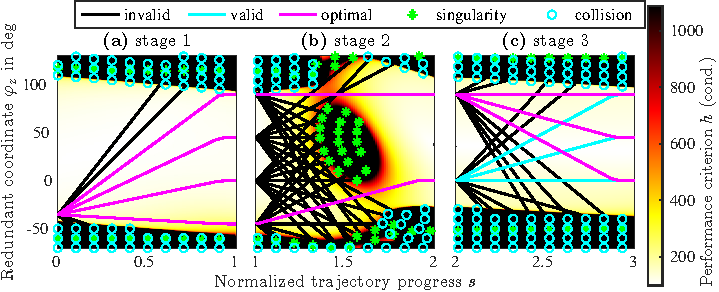
\includegraphics{dp_discr_stage1_to_3_compressed.pdf}
\caption{Decisions on the first three stages using discrete DP for the reference problem}
\label{fig:dp_example_stage1}
\end{figure}


\begin{figure}[tb]
\centering
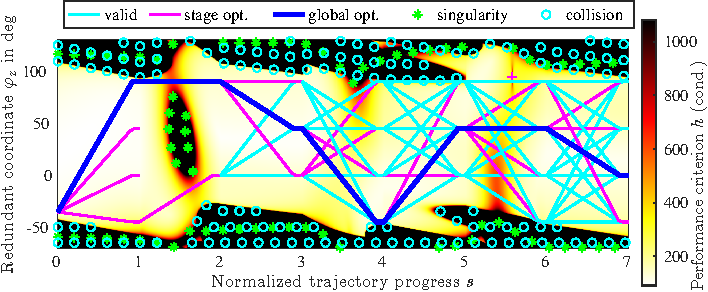
\includegraphics{dp_discr_result_compressed.pdf}
\caption{Result of discrete dynamic programming for the reference problem}
\label{fig:dp_example_all}
\end{figure}

The final result of the algorithm after performing the remaining stages $k=4...7$ is shown in Fig.~\ref{fig:dp_example_all} with the highlighted optimal trajectory that has been found.
The continuous optimization variable can only very roughly be approximated by the chosen discretization of $\varphi_{z} = \SI{45}{\degree}$.
Choosing a finer discretization is able to improve the result in this case, but using the discrete DP is not applicable to the general case, if a feasible solution can not be found via straight lines in the performance map.
Further, the DP algorithm has complexity $\mathcal{O}(n n_{\mathrm{ref}}^2)$, making the presented implementation inefficient for such continuous problems.


\subsection{State-Interval Dynamic Programming}
\label{sec:trajopt_dp_interval}

The drawbacks of the classical discrete dynamic programming can be solved by defining a target interval for the states rather than a fixed value.
A state interval 
\begin{equation}
[x] = [\bar{x}-\nicefrac{\Delta x}{2}, \bar{x}+\nicefrac{\Delta x}{2}]
\end{equation}
is defined by a center $\bar{x}$ and the interval width $\Delta x$.
Instead of a fixed set of discretized reference states $X_\mathrm{ref}$ in (\ref{equ:dp_refstate}), the states are now\footnote{Intervals are assumed non-overlapping (i.e. half-open) for the sake of mathematical proof, however the symbol $[\cdot]$ for closed intervals is used to enhance readability.} 
\begin{equation}
X_\mathrm{ref}=
\{
[x_{\mathrm{ref},1}],[x_{\mathrm{ref},2}],...,[x_{\mathrm{ref},n_{\mathrm{ref}}}]
\}.
\end{equation}
The DP formulation from the previous section is adapted in such a way that previous states remain specific values $x_{k-1}$.
Future states are considered as an interval, allowing a set of solutions $x_{k} \in [x_{k}]$ or $\bar{x}_{k}{-}\nicefrac{\Delta x}{2} \le x_{k} < \bar{x}_{k}{+}\nicefrac{\Delta x}{2}$.
%
The set of decision variables from (\ref{equ:dp_decisionset}) now becomes

\begin{equation}
U_k(x_{k-1}) = 
\begin{cases} 
\emptyset & \mathrm{for} \enspace  J^*_{k}(x_{k-1}) = \infty \\
\{ u_k 
\enspace | \enspace 
f(x_{k-1},u_k) \in [x_k] 
\enspace \forall \enspace 
[x_k] \in X_k
\}
& \mathrm {otherwise.} \vspace{-0.3cm} % to reduce distance to equ. number
\end{cases}
\label{equ:idp_decisionset}
\vspace{0.2cm} % distance to text to counter negative vspace from above
\end{equation}


Since the intervals do not overlap, Bellman's principle of optimality still holds under the assumption of an optimal state transfer regarding the subproblem in $f(x_{k-1},u_k)$.
This means that the transfer to the actual reached state $x_k$ within the interval $[x_k]$ is assumed to be optimal among all possible local transfer strategies $\tilde{u}_k$, i.e.
\begin{equation}
l_k(x_{k-1},u_k) = \min_{\tilde{u}_k}{\{
l_k(x_{k-1},\tilde{u}_k)
\enspace \forall \enspace
\tilde{u}_k
\enspace |  \enspace
f(x_{k-1},\tilde{u}_k) \in [x_k]
\}}.
\label{equ:idp_localopt}
\end{equation}
The transition strategy $u_k$ in this case is not only correspondence to a target state $x_k$, but also a specific control strategy for the subproblem $f(x_{k-1},u_k)$. 
In the trajectory optimization example this includes the optimal decision for each of the dense trajectory samples, as mentioned in Sect.~\ref{sec:problem_differential}.
The assumption (\ref{equ:idp_localopt}) is unlikely to strictly hold in the presented highly nonlinear robot application.
However, approximating this by a near-optimal or at least feasible $u_k$ may already be enough to obtain acceptable results regarding difficulties in finding valid solutions at all, facing the constraints. 

The decision $u_k$ now only has to assure that the next state lies in it's allowed interval.
This improves the possibility to perform a local optimization in the state transfer function, which corresponds to the trajectory optimization via the nullspace projection.
Reaching the interval has to be implemented with extensions to the local optimization or with constraints, as discussed in Sect.~\ref{sec:trajik_perf}.

The backward recursion from (\ref{equ:dp_backward}) using the interval approach now is
\begin{equation}
J^*_{k}([x_k]) = \min{\{J_k(x_{k-1},u_k) 
\enspace | \enspace 
f(x_{k-1},u_k) \in [x_k] \land u_k \in U_k(x_{k-1})  \}}.
\label{equ:idp_backward}
\end{equation}
%
The cumulated cost $J_k(x_{k-1},u_k) $ does not change compared to (\ref{equ:dp_cumcost}), since looking retrospectively, the previous state $x_{k-1}$ is the actual obtained value, no interval.

The proposed approach is illustrated at the previous robot trajectory example.
Interval limits are set as before as 
$x_{\mathrm{ref},1}=\varphi_{z,\mathrm{min}}=\SI{-180}{\degree}$, $x_{\mathrm{ref},n_{\mathrm{ref}}}=\varphi_{z,\mathrm{max}}=\SI{180}{\degree}$,  $n_{\mathrm{ref}
}=9$, $\Delta x = \Delta \varphi_{z} = \SI{45}{\degree}$ and  $x_0=\varphi_{z,0}\approx\SI{-35}{\degree}$.
The term $x_{\mathrm{min}}$ and $x_{\mathrm{max}}$ is not used since the limits for the optimization variable are extended by the interval half-span $\Delta x / 2$.
A decision $u_k$ consists of a reference trajectory as in the previous discrete DP example.
This trajectory is only tracked via a feed-forward gain and a nullspace controller, as explained in Sect.~\ref{sec:taskred}.
A tolerance band around the trajectory ensures reaching the respective target interval $[x_k]$, as shown in Fig.~\ref{fig:idp_example_stage1} for three exemplary decisions on the first stage.

\begin{figure}[ptb]
\centering
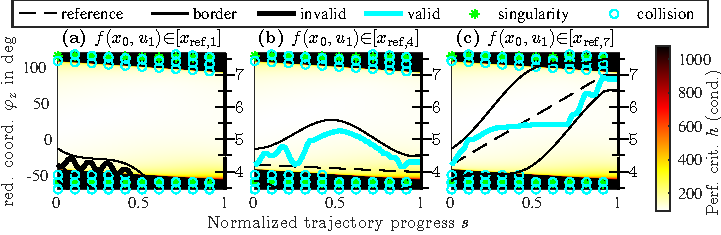
\includegraphics{dp_interv_stage1_3cases_compressed.pdf}
\caption{Decisions $u_1$ on the first stage using state-interval dynamic programming to exemplary state intervals 1 \textbf{(a)}, 4 \textbf{(b)} and 7 \textbf{(c)} on stage 2. The numbers $i$ on the axis to the right of each performance map correspond to the state intervals $[x_{\mathrm{ref},i}]$ }
\label{fig:idp_example_stage1}
\end{figure}

\begin{figure}[ptb]
\centering
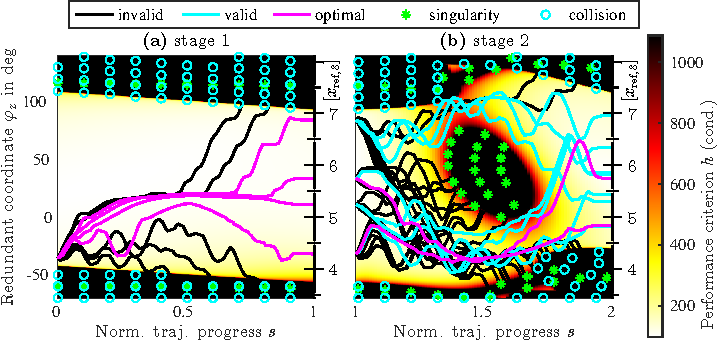
\includegraphics{dp_interv_stage1_to_2_compressed.pdf}
\caption{All decisions on the first two stages using state-interval DP}
\label{fig:idp_example_stage12}
\end{figure}

\begin{figure}[ptb]
\centering
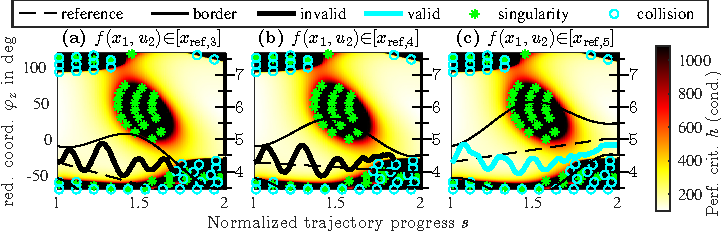
\includegraphics{dp_interv_stage2_3cases_compressed.pdf}
\caption{Decisions $u_2$ on the second stage from $x_1 \in [x_{\mathrm{ref},4}]$ using state-interval DP}
\label{fig:idp_example_stage2}
\end{figure}


\begin{figure}[ptb]
\centering
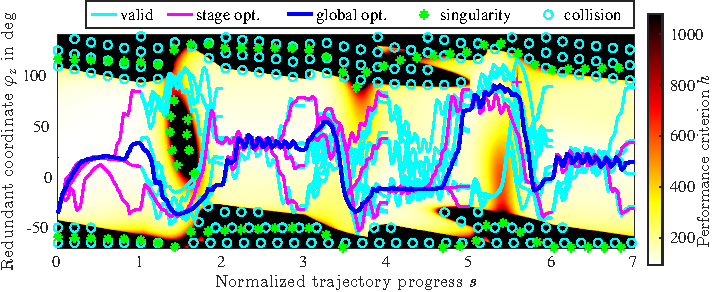
\includegraphics{dp_interv_result_compressed.pdf}
\caption{Result of state-interval dynamic programming for the reference problem}
\label{fig:idp_example_all}
\end{figure}

As in the previous example, not all target states lead to valid results, especially since the global distribution of the performance map is not known in advance and therefore a wide span is chosen.
All transitions of the first stage are shown in Fig.~\ref{fig:idp_example_stage12},a.
The valid lines are continued in the next stage.
Since only one starting state exists, all valid lines are also optimal, which is highlighted by the color magenta.
The continuation for stage 2 is shown first exemplarily together with the reference trajectory and spline-based tolerance intervals in Fig.~\ref{fig:idp_example_stage2}.
Figure.~\ref{fig:idp_example_stage12},b contains all transfers.
Multiple decisions $u_1$ lead to the same state intervals of $[x_2]$, as visible for the cyan lines ending in $[x_{\mathrm{ref},5}]$ and $[x_{\mathrm{ref},6}]$ (noted by the numbers at the right side of Fig.~\ref{fig:idp_example_stage12},b).
Therefore the best decisions according to (\ref{equ:idp_backward}) are selected for continuation, marked magenta.
The result of the algorithm is depicted in Fig.~\ref{fig:idp_example_all}.

\subsection{Overlapping Intervals}
\label{sec:overlapping}

The approach presented above enforces the redundant coordinate in a tolerance band by using a repulsing potential $h_{\varphi_{z},\mathrm{lim}}$.
This has the effect that a local optimum on this border between intervals can not be reached.
A solution to achieve this is the use of overlapping intervals.
It still has to be assured, that at each stage only the prescribed number of state intervals are continued.
Otherwise the number of states will grow from state to state and the underlying optimality principle of dynamic programming does not hold any more.
The extension leads to additional possible decisions on each set, extending the set $X_k$ in (\ref{equ:idp_decisionset}) to
%
\begin{equation}
X_\mathrm{k}'=
\{
[x_{\mathrm{ref},1}],[x_{\mathrm{ref},2}],...,[x_{\mathrm{ref},n_{\mathrm{ref}}}],
[x_{\mathrm{add},1}],...,[x_{\mathrm{add},n_{\mathrm{add}}}]
\}.
\label{equ:idp_decisionset_ol}
\end{equation}
%
The additional intervals are set to be overlapping with the existing ones, i.e.
%
\begin{equation}
[x_{\mathrm{add},k}]=[x_{\mathrm{ref},k}]+\nicefrac{\Delta x}{2}
= x_{\mathrm{ref},k} \le x <  x_{\mathrm{ref},k+1}
\end{equation}
%
and $n_{\mathrm{add}}=n_{\mathrm{ref}}-1$.
To prevent the number of states from increasing, the cumulated cost in the backward recursion (\ref{equ:idp_backward}) is not evaluated for the new, overlapping intervals from (\ref{equ:idp_decisionset_ol}).

\subsubsection{Robot Trajectory Example:}
The modification of overlapping intervals is again demonstrated at the robot example.
The chosen parameters are now $n_\mathrm{ref}=5$ with $\Delta x = \Delta \varphi_{z} = \SI{90}{\degree}$.
Due to the overlapping intervals, the number of forward iterations stays the same, but fewer states are considered for continuation.
Similar to Fig.~\ref{fig:idp_example_stage1}, the first stage transfer is investigated in Fig.~\ref{fig:idp_ol_example_stage1}.
The transfer in Fig.~\ref{fig:idp_ol_example_stage1},c corresponds to the additional interval $[x_{\mathrm{add},3}]$ between $[x_{\mathrm{ref},3}]$ in Fig.~\ref{fig:idp_ol_example_stage1},a and $[x_{\mathrm{ref},4}]$ in Fig.~\ref{fig:idp_ol_example_stage1},b.

\begin{figure}[ptb]
\centering
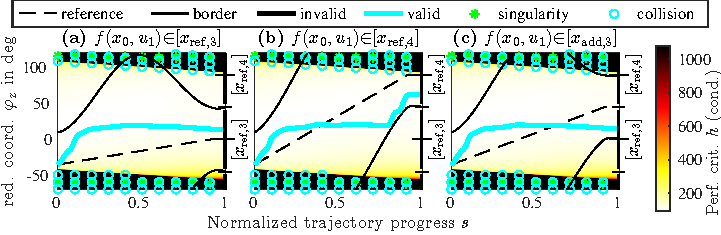
\includegraphics{dp_interv_overlap_stage1_3cases_compressed.pdf}
\caption{Decisions $u_1$ on the first stage using overlapping state-intervals in dynamic programming to exemplary state intervals 3 \textbf{(a)}, 4 \textbf{(b)} and the overlapping interval in-between \textbf{(c)} on stage 2}
\label{fig:idp_ol_example_stage1}
\end{figure}

Similar to Fig.~\ref{fig:idp_example_stage12} all transfers on the first two stages are shown in Fig.~\ref{fig:idp_ol_example_stage12}.
Transfers from additional overlapping intervals are marked with dashed lines.
Now already in the first stage in Fig.~\ref{fig:idp_ol_example_stage12},a multiple actions lead to a transfer to the interval $[x_{\mathrm{ref},3}]$, which seemingly contains the local optimum.
The best of these is selected in stage 2 (Fig.~\ref{fig:idp_ol_example_stage12},b) for continuation.

\begin{figure}[ptb]
	\centering
	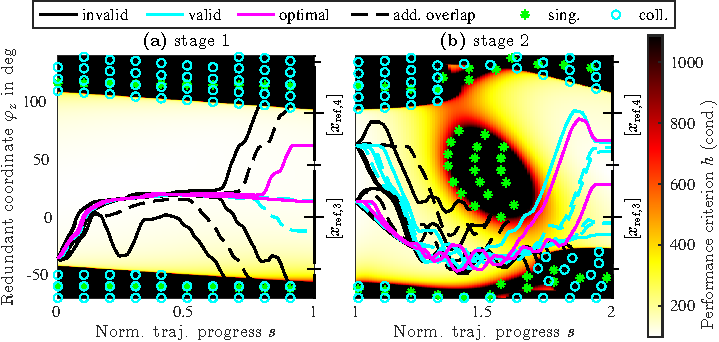
\includegraphics{dp_interv_overlap_stage1_to_2_compressed.pdf}
	\caption{Decisions on stage 1 and 2 for the reference problem using overlapping intervals}
	\label{fig:idp_ol_example_stage12}
\end{figure}

\section{Simulative Validation for a Parallel Robot}
\label{sec:eval}

In the following a quantitative evaluation of the proposed new method of state-interval dynamic programming (SI-DP) from Sect.~\ref{sec:trajopt_dp_interval} is performed with a comparison against classical dynamic programming (DP) from Sect.~\ref{sec:trajopt_dp_discr} and the previous approach of local optimization using nullspace projection (NP) from Sect.~\ref{sec:taskred} (and \cite{SchapplerOrt2021}).
An overview of robot and task can be obtained from Fig.~\ref{fig:teaser_image}.
The same benchmark task as in the previous section is used.
The robot has the following dimensions: base diameter \SI{1200}{\milli\metre}, platform diameter \SI{300}{\milli\metre} and distance of hexagonally aligned platform coupling joint pairs of \SI{100}{\milli\metre}.
Collision bodies for the leg chains have a diameter of \SI{40}{\milli\metre}.
The task is beginning at $[r_x, r_y, r_z]=[-50, 40, 700]$\,mm and $[\varphi_x, \varphi_y]=[45^\circ,0^\circ]$ in the robot base frame and has a length of \SI{900}{\milli\metre} and duration of \SI{31.6}{\second} with seven rest poses.
The trajectory has 31647 samples with a sample time of \SI{1}{\milli\second}. 

\begin{figure}[tb]
\centering
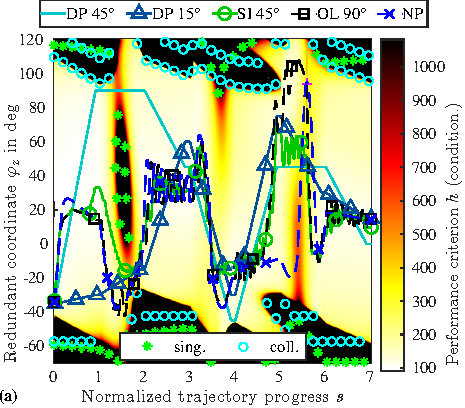
\includegraphics{nullspace_traj1_compressed.pdf}
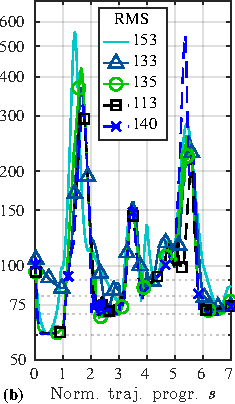
\includegraphics{nullspace_traj1_condition.pdf}
\caption{Nullspace motion in performance map \textbf{(a)} and evolution of criterion \textbf{(b)}}
\label{fig:eval_example1}
\end{figure}

The comparison in Fig.~\ref{fig:eval_example1} shows that the SI-DP with a discretization of \SI{45}{\degree} outperforms the classical discrete DP with the same discretization in the critical phases of the trajectory.
Further, DP presents a different trajectory with $\varphi_z{=}$\SI{90}{\degree} at $s{=}2$ due to the narrow passage.
The reason can be found in the only very rough discretization, which is beneficial for the SI-DP and reduces computation time.
A further improvement is achieved by using the overlapping (OL) intervals from Sect.~\ref{sec:overlapping} with discretization of \SI{90}{\degree}.
The evaluation of one trajectory sample needs \SI{0.4}{\milli\second} for the DP and \SI{1.2}{\milli\second} for the SI-DP and OL-SI-DP, due to more complex nullspace equations.
A Linux desktop computer with Intel i5-7500 CPU and \textsc{Matlab} implementation using \textsc{mex}-compiled functions was used.
The total optimization for DP with \SI{45}{\degree} took \SI{3.4}{\minute} with 535k trajectory samples, corresponding to 16.9 times the full trajectory length.
%This shows the necessity of the abortion at constraint violations, since without abortions $(n_{\mathrm{ref}} + (n-1) \times n_{\mathrm{ref}}^2)/n=(9+6\times 81)/7=59$ equivalents of the full trajectory would have to be computed.
The SI-DP with \SI{45}{\degree} took \SI{13.2}{\minute} for 664k samples, i.e. 21 full trajectory equivalents and the OL-SI-DP took \SI{10}{\minute} for 421k samples.
The RMS value according to (\ref{equ:h_integral}) is given in Fig.~\ref{fig:eval_example1},b and shows the improved performance by the SI-DP by a value of 135 and OL by 113.
The DP results can be improved by finer discretization of \SI{15}{\degree}, which leads to a similar RDP value of 134 like SI-DP, instead of 153, but takes \SI{25.7}{\minute} for 4M samples, i.e. 128 full trajectory equivalents.

The NP method performs better in the first two phases since the optimal solution is between intervals of the SI-DP, which is a repulsing potential.
Using the OL method solves this problem.
The only local optimality of NP becomes visible at $s{=}5$ where a local optimum is followed by a region of high cost terms, which has to be traversed.
This leads to a moderately worse RMS value of 140, but needs the least computational effort with \SI{39}{\second} for one full trajectory.


The example is modified in the following to pose higher restrictions on the robot.
The trajectory length is increased to \SI{1400}{\milli\metre} and the pointing direction now is \SI{45}{\degree} to the outside, i.e. $[r_x, r_y, r_z]=[-200, 150, 700]$\,mm and $[\varphi_x, \varphi_y]=[-45^\circ,0^\circ]$ for the starting point.
The robot is shown in Fig.~\ref{fig:example2_robot} for three different points of this second trajectory.
The cases of singularity and collision are highlighted for illustration.
The trajectory optimization is performed with the same methods and settings as before with results presented in Fig.~\ref{fig:eval_example2}.
Due to the very narrow passages of possible rotation angle $\varphi_z$, the \SI{45}{\degree}-DP does not find a solution, as well as the local optimization.
The fine-discretization \SI{15}{\degree}-DP and the proposed \SI{45}{\degree}-SI-DP find a solution, where SI-DP outperforms the DP by means of RMS of the condition number and OL performs best due to less constraints for enforcing the interval.


\begin{figure}[htb]
\centering
\input{./figures/traj2_overview_cases.pdf_tex}
\vspace{-0.3cm}
\caption{Robot in three poses of the second performance map example from Fig.~\ref{fig:eval_example2}}
\label{fig:example2_robot}
\end{figure}

\begin{figure}[htb]
\centering
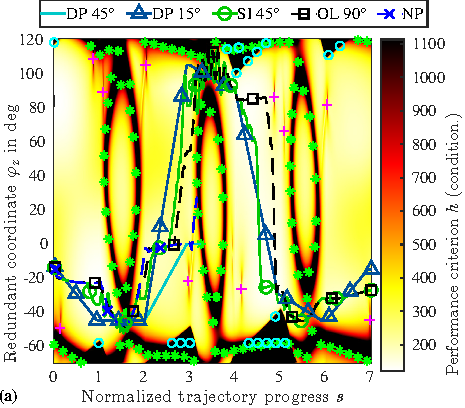
\includegraphics{nullspace_traj2_compressed.pdf}
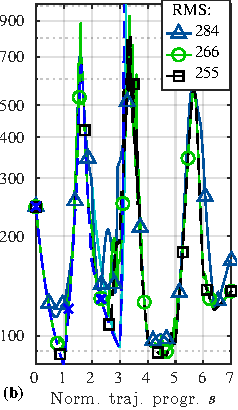
\includegraphics{nullspace_traj2_condition.pdf}
\vspace{-0.3cm}
\caption{Results for the second example: Performance map \textbf{(a)} and criterion \textbf{(b)}}
\label{fig:eval_example2}
\end{figure}

For both examples oscillations can be observed in Fig.~\ref{fig:eval_example1} and Fig.~\ref{fig:eval_example2} for the nullspace optimization methods SI-DP, OL-SI-DP and NP.
This could be omitted by further tuning of PD gains and damping.
However at least for SI-DP the oscillation is partially inherent to the method since a repulsing potential from the coordinate limits is used.

\section{Conclusion}
\label{sec:conclusion}

The presented algorithm corresponds to a combination of differential and classical dynamic programming and is applicable to trajectory optimization problems of dynamic systems with continuous state and stage variables and rest-to-rest state transitions.
The performance measure in intermediate steps should have a correlation with the global optimization objective.
This can be the case by globally optimizing the average values of local objectives and in the presence of high penalties for constraints.
An example of a robot trajectory optimization is given, however similar problems may arise in other disciplines as well.
The results show the improved performance compared to discrete DP or local optimization at acceptable computation times for offline trajectory planning.
The approach is not restricted to second-order trajectories or task redundancy within robotics.
Optimizing multiple redundant degrees of freedom is also possible, but without the performance map visualization used throughout the paper.
Instead of nullspace optimization, also other local optimization techniques could be used, which leads to a still open future investigation on conditions for the analogy of the proposed method to existing ones like DDP.
%A systematic classification of the method compared to the plurality of existing methods for local and global optimization still remains.
%The next application within the inverse kinematics will be the dimensional synthesis.
%Further evaluations may include optimizing CNC machining trajectories with a high amount of single motions.

\subsubsection{Acknowledgements} The author acknowledges the support by the Deutsche Forschungsgemeinschaft (DFG) under grant number 341489206.
\textsc{Matlab} Code to reproduce the results is available at GitHub under free license at\\ \url{https://github.com/SchapplM/robotics-paper_icinco2021}.

%
% ---- Bibliography ----
%

\bibliographystyle{splncs04}
\bibliography{references}

\end{document}
